\chapter{Experiments}
\label{ch:experiments}


\section{Machine properties}
Within the experiments it was used macbook pro middle 2018 with Coffee Lake/8th generation: a 2.2GHz Core i7 processor with six cores and with intel turbo boost up to 4.1GHz.

\section{Data}
The experimental \ref{fig:ct_spine} data set was splitted into dedicated training (with ground-truth labels) and test sets each 242 and 60 scans accordingly. The scans were re-sample  at 1mm x 1mm x 1mm resolution meaning each pixel in the generated samples from the scans provided a 3 dimensional 1mm section of the patient spine.
\begin{figure}[h]
    \centering 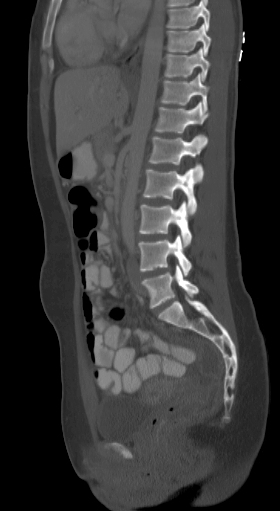
\includegraphics[width=3cm]{images/ct-spine.jpg}
    \caption {Train sample of CT spine scan}
    \label{fig:ct_spine}
\end{figure}


\section{Training detection model}
trained for 50 epochs which took 11 hours. obtained a validation Dice score of 0.961 on the 1 (vertebrae) labels and a validation accuracy of 98.5 on test samples generated from test set.
At test time applied the detection model to a scan patch-wise with some overlap between patches. The input to the network is 64 x 64 x 80 and we applied it in steps of 32 x 32 x 40, padding the border of the scan by 16 x 16 x 20 and discarding the outer border of size 16 x 16 x 20 from each output. This reduced edge artifacts in the detection and led to improved mean localization scores.

\section{Training identification model}
trained for 35 epochs which took 7 hours.
The identification model is a fully convolutional network which allows us to apply it to whole slices of the input scan, padded to the nearest multiple of 16, at test time.


\section{Results}
results are calculated over the dedicated testing set of
60 scans. measured metrics, Id rate, mean localization distance and standard deviation (std) distance. Id rate is the percentage of the centroid estimations predicted which are closest to the correct ground truth vertebra centroid (and are less than 20mm from that centroid). Mean and Std relate to the localization error distance between the predicted centroid positions and the ground-truth centroid positions for the same vertebrae (if it occurs in the scan).

%
- competitors

%
- table of comparison